\style{mbot}
%   Titre de la sous sections
\section{Vitesse de rotation avec MBot}



\subsection{Description}

\subsubsection{Objectif}


%   bloc de formule
%   sans titre et fond bleu cyan
\begin{formule}
L'objectif du projet est de mettre en évidence, par l'expérimentation, l'influence du diamètre d'une roue sur la vitesse linéaire d'un véhicule.

Il faut arriver à observer que, pour un même distance,  l'augmentation du diamètre des roues entraîne une diminution du temps de parcours du véhicule.

Autrement dit : la vitesse linéaire augmente lorsque le diamètre des roues augmente
\end{formule}


\subsubsection{Intérêt}

Il est intéressant d'aborder le thème de sciences \textit{Comment passer de la vitesse des roues à la vitesse du véhicule} avec un robot. En effet :

%liste d'arguments
\begin{description}
    \item [Expérimentation et démarche scientifique] l'élève manipule tout au long de l'activité, fait des hypothèses et doit valider ses choix
    \item [Objet attrayant] le robot Mbot reste attractif pour les élèves et sa programmation permet de valoriser le travail de l'élève
\end{description}


\subsubsection{Matériel}
\begin{itemize}

%   matériel pour MBot
    \item 1 $\times$ \matosMbot
%   site internet pour MBot
   \item 1 $\times$ accès internet : IDE programmation par bloc \url{http://editor.makeblock.com/ide.html}
    
\end{itemize}



\subsubsection{Remarques}


%   bloc méthode
%   titre + fond bleu
\begin{methode}
    L'activité propose de mettre en évidence le lien entre variation du diamètre et variation de vitesse linéaire.
    
    Cette activité peut être prolongée par une vérification de la relation entre vitesse linéaire ($V$), rayon ($r$) et fréquence de rotation ($N$) : $V = 2 \times \pi \times r \times N$.
    
    Pour cela il faudra utiliser un \textbf{tachymètre} permettant une mesure de la fréquence de rotation.
    
\end{methode}

%
% activité de niveau 
%

%   saut de page
\newpage

%   titre de la sous section
\subsection{Niveau initiation}

\subsubsection{Activité élève}

% commande perso \CARTOUCHE
%   5 paramètres : 
%       * durée
%       * public
%       * travail en maths
%       * travail en sciences
%       * travail en algo
\cartouche
{2 h}         %durée
{2de}           %public
{}        %maths
{mouvement, durée, distance, vitesse linéaire}     %sciences
{instructions déplacement}       %algo


%   petite image de logo qui va
%   se mettre dans le bloc élève
\begin{wrapfigure}[5]{r}{3cm}
    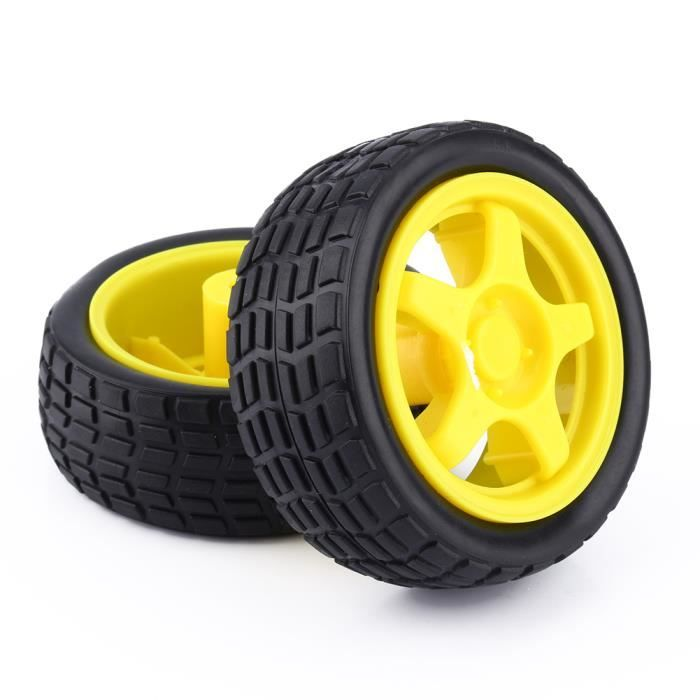
\includegraphics[width=\linewidth]{res/mbot100.jpg}
\end{wrapfigure}

%   bloc élève
%   fond orange
\begin{eleve}

Hélias veut booster son robot en changeant les roues. Il a trouvé sur Internet de jolies roues jaunes pouvant s'adapter sur le MBot.

Ces nouvelles roues sont plus grandes et Hélias s'exclame : \textit{"En plus, lorsque je sélectionnerai la vitesse 100, mon robot ira plus vite !"}.

    \texttt{\textsc{Ta Mission} : 
    Comment vérifier si Hélias a raison, le robot ira-t-il vraiment plus vite ?
    }
%   ajout d'une image
%    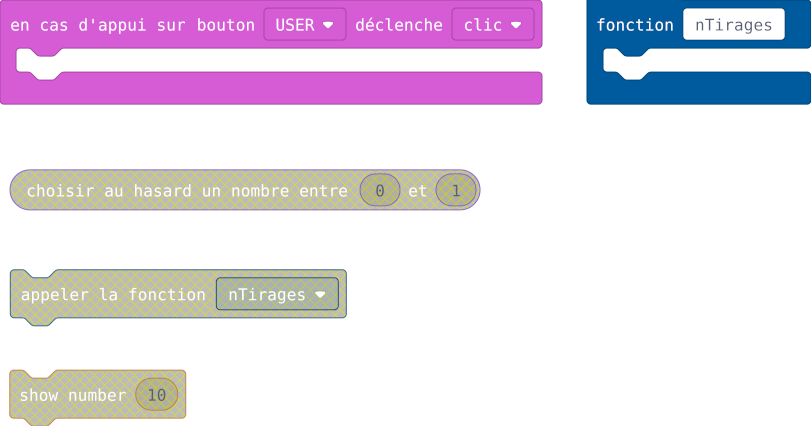
\includegraphics[width=0.5\linewidth]{res/st-pf-00-eleve.png}
\end{eleve}



\subsubsection{Notes pour l'enseignant}

%
%   méthode et remarque
%

\begin{minipage}[t]{0.5\linewidth}
    \begin{methode}~\\
     \begin{enumerate}
         \item La distance doit être \textbf{suffisamment grande} pour mettre en évidence la variation de vitesse et \textbf{suffisamment petite} pour éviter une dérive du robot.
        \item Montrer l'intérêt de faire plusieurs fois la \textbf{même mesure} afin de mettre évidence la variabilité d'une mesure.
        \item Proposition de code :
     \end{enumerate}
        ~\\
        \begin{center}
            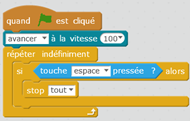
\includegraphics[width=0.85\linewidth]{res/mbot-vitesse-sol.png}
        \end{center}
    \end{methode}
\end{minipage}
\hfill
\begin{minipage}[t]{0.5\linewidth}
    \begin{remarque}~\\
        Les élèves utilisent leur téléphone (pour mesurer le temps) et une règle (pour déterminer une distance).
        
        L'utilisation de la barre d'espace pour arrêter le robot n'est pas indispensable mais est \textbf{très pratique} pour gérer l'arrêt du robot.
    \end{remarque}
\end{minipage}